\chapter{Design and Analysis}

\section{Introduction}

Chapter 2 discussed the theoretical background and literature related to EO/IR aerial segmentation. This chapter presents the design and analysis of the experimental framework used in this dissertation. The purpose of the framework is to study how YOLO-based segmentation models behave under different EO/IR training conditions and to identify which design choices most improve IR-domain segmentation quality.

The experimental design follows a controlled progression. First, EO-only baselines are used to measure the direct EO-to-IR domain gap. Next, grayscale-domain transformations are applied to EO data to test whether reducing visible color bias improves IR generalization. After that, real IR supervision is introduced through IR-only and EO+IR mixed-domain training. The study then evaluates the effect of model scaling, high-resolution training, and mask-aware ensembling. This design allows each major factor to be analyzed separately.

Figure \ref{fig:proposed_workflow} summarizes the proposed workflow used to organize the dataset preparation, experiment groups, model training, evaluation, and result consolidation stages.

\begin{figure}[htbp]
\centering
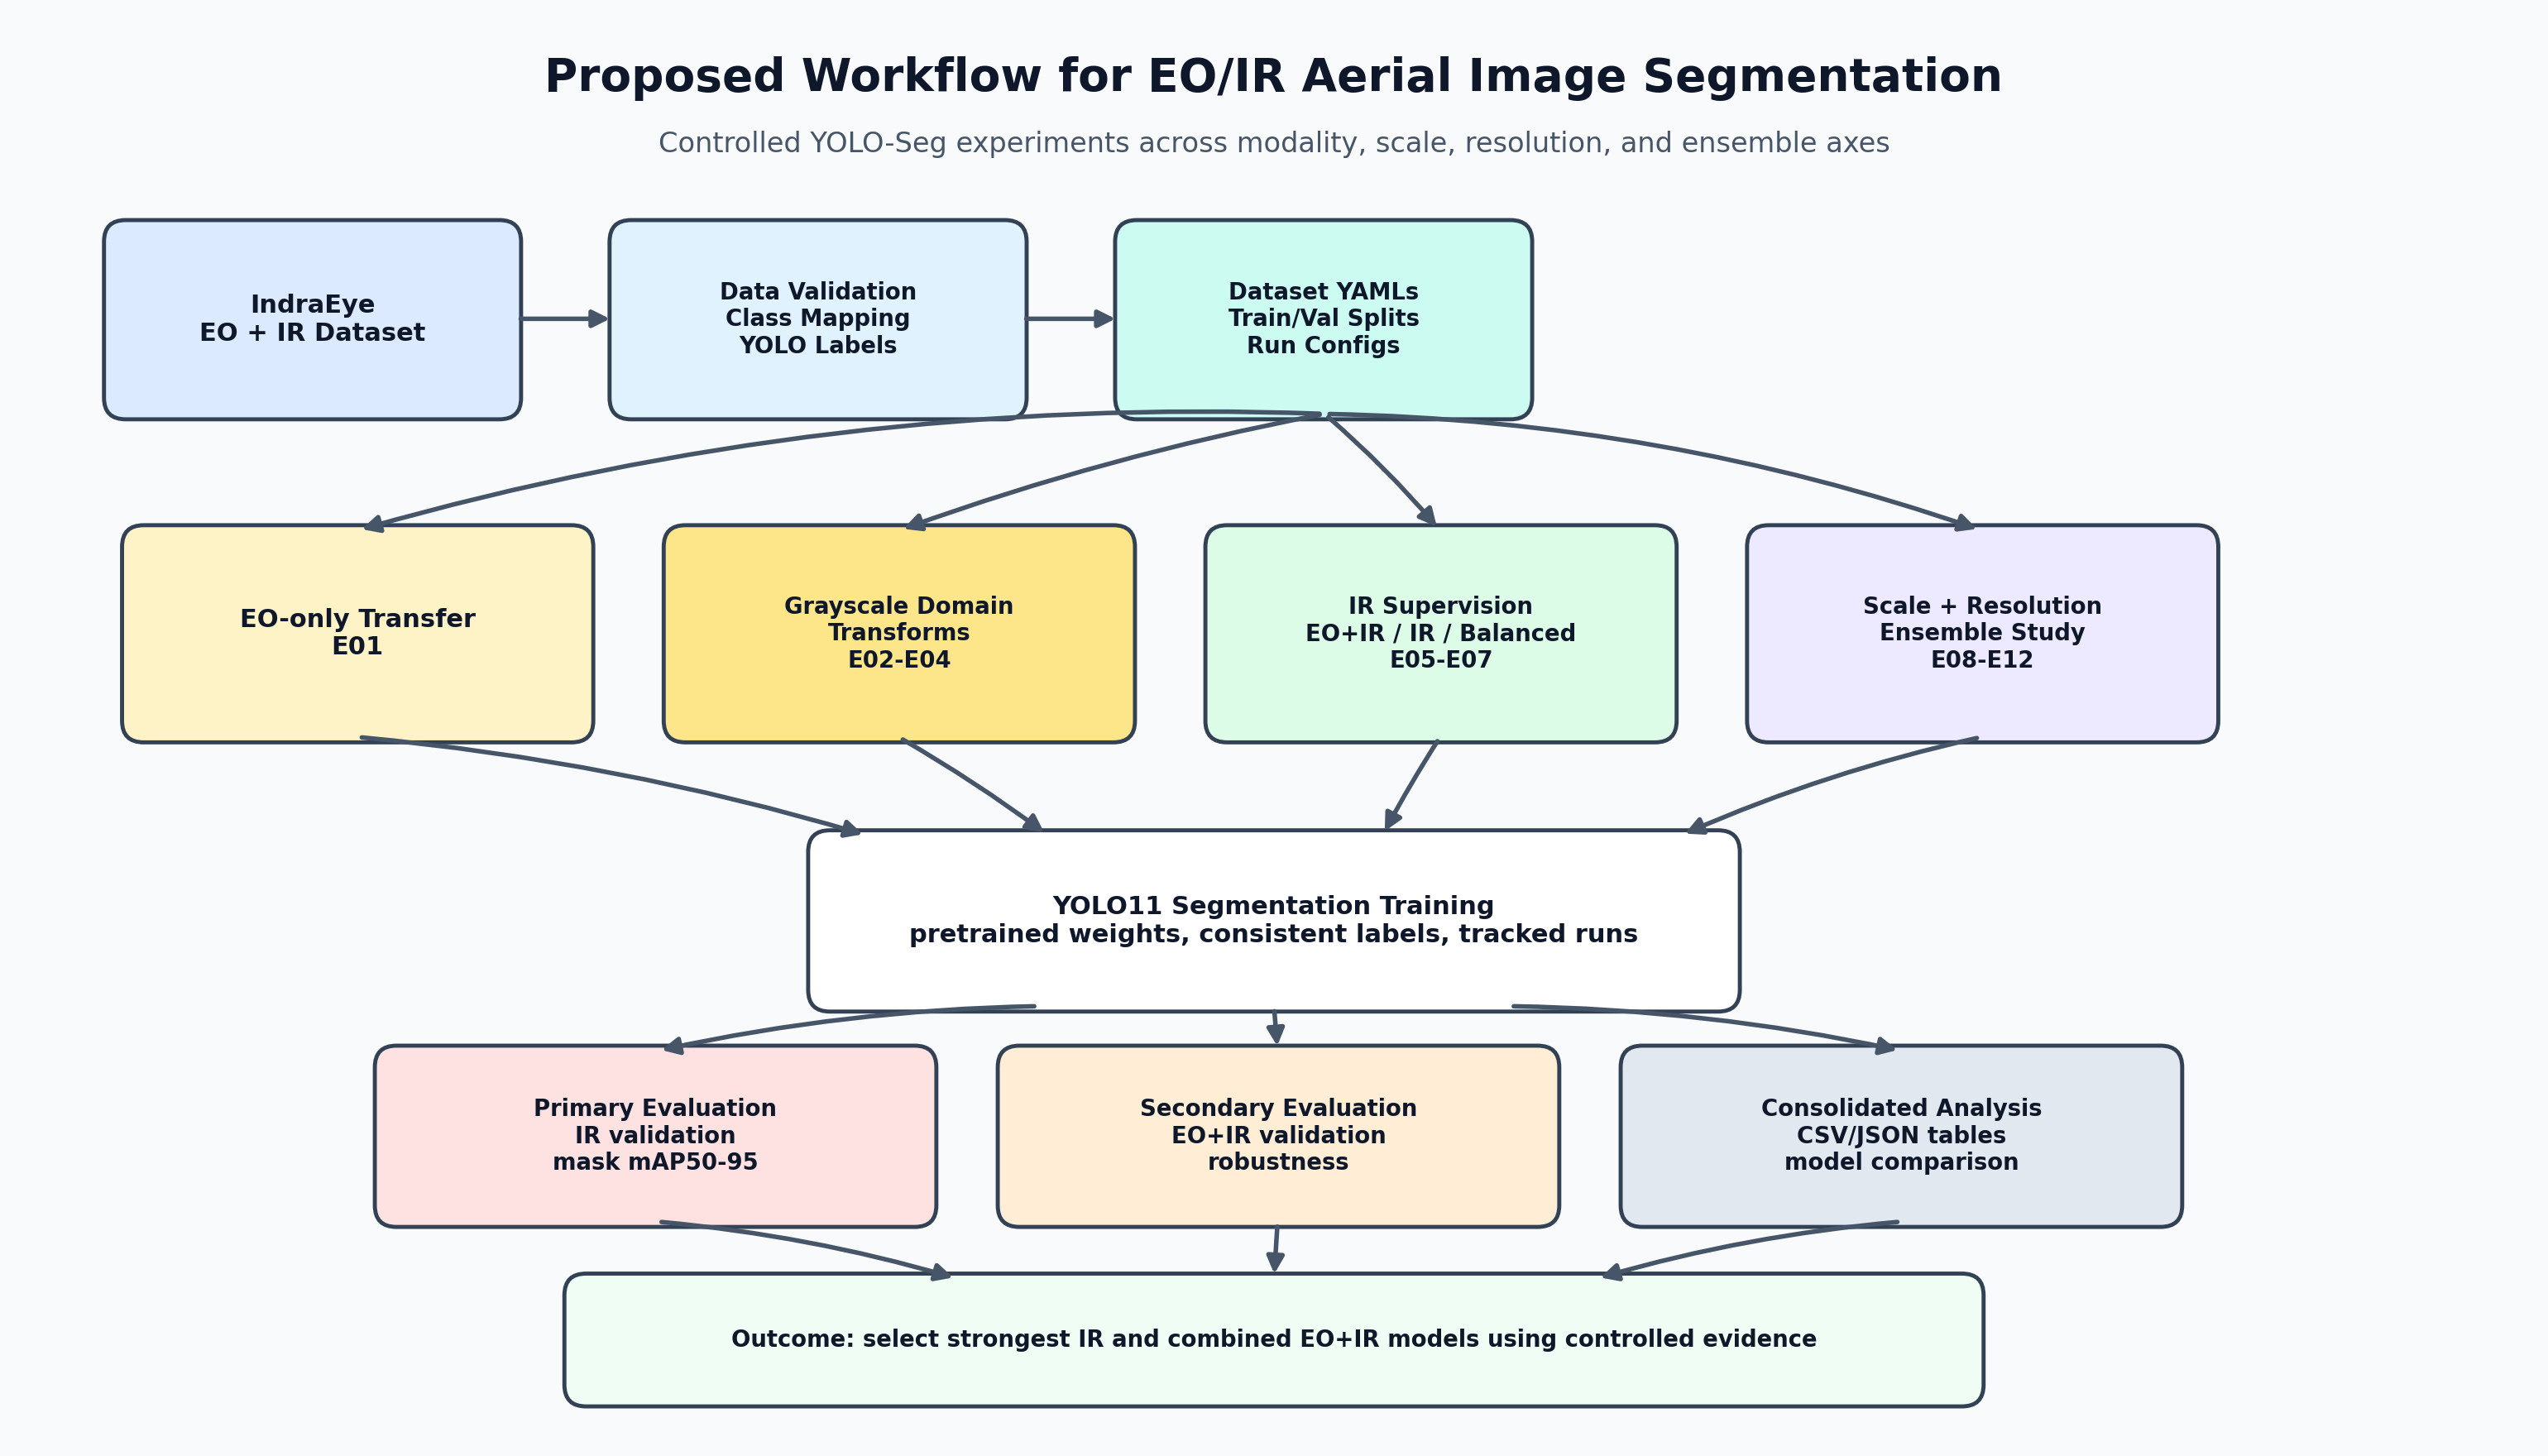
\includegraphics[width=\textwidth]{Figures/Chapter3/proposed_workflow.png}
\caption{Proposed workflow for the EO/IR aerial image segmentation study.}
\label{fig:proposed_workflow}
\end{figure}

\section{Design Goals}

The proposed framework was designed with the following goals:

\begin{enumerate}
    \item To establish a reproducible YOLO segmentation workflow for EO/IR aerial traffic imagery.
    \item To separate EO-only domain-transfer experiments from supervised IR and EO+IR experiments.
    \item To evaluate whether grayscale-domain transformations are sufficient for IR segmentation.
    \item To measure the effect of adding real IR training labels.
    \item To study the effect of YOLO model capacity on segmentation performance.
    \item To study the effect of higher input resolution on small-object mask quality.
    \item To evaluate whether model ensembling improves beyond strong single-model baselines.
    \item To maintain consistent evaluation settings across all experiments.
\end{enumerate}

The main design principle is controlled comparison. Each experiment changes one main factor while keeping the remaining evaluation protocol as consistent as possible. This makes it easier to interpret whether an improvement is caused by data modality, augmentation, model scale, resolution, or ensembling.

\section{Dataset Organization}

The dataset used in this dissertation is organized into two sensing modalities: EO and IR. Each modality contains images and labels for training and validation. The expected directory structure is:

\begin{verbatim}
eo/
  images/train
  images/val
  labels/train
  labels/val
ir/
  images/train
  images/val
  labels/train
  labels/val
\end{verbatim}

The labels are stored in YOLO segmentation format. Each label file contains object class identifiers and polygon coordinates corresponding to object masks. The same class mapping is used across EO and IR data so that models can be trained and evaluated consistently across modalities.

\section{Class Taxonomy}

The active class set contains twelve class identifiers. The class mapping is shown in Table \ref{tab:class_mapping}.

\begin{table}[h]
\centering
\caption{Class mapping used for YOLO segmentation experiments.}
\label{tab:class_mapping}
\begin{tabular}{cl}
\hline
\textbf{Class ID} & \textbf{Class Name} \\
\hline
0 & Bicycle \\
1 & Bus \\
2 & Car \\
3 & Cargo trike \\
4 & Ignore \\
5 & Motorcycle \\
6 & Person \\
7 & Rickshaw \\
8 & Small truck \\
9 & Tractor \\
10 & Truck \\
11 & Van \\
\hline
\end{tabular}
\end{table}

The class set reflects traffic participants and vehicle types commonly observed in Indian aerial road scenes. The \texttt{Ignore} class is retained in the label structure but is not treated as a semantic foreground object during object-region grayscale augmentation.

\section{Evaluation Design}

Two validation settings are used throughout the study:

\begin{enumerate}
    \item \textbf{IR-only validation:} This setting evaluates a trained model only on the IR validation split. It is referred to as \texttt{eval\_ir}. This is the primary evaluation setting because the main objective is to improve IR segmentation quality.
    \item \textbf{Combined EO+IR validation:} This setting evaluates a trained model on a combined validation set containing both EO and IR validation images. It is referred to as \texttt{eval\_eo\_ir}. This setting measures cross-modality robustness.
\end{enumerate}

The primary metric is mask mAP50-95. This metric is stricter than mask mAP50 because it averages performance across multiple IoU thresholds. Since the dissertation focuses on segmentation masks, strict mask quality is more important than coarse localization alone. Box metrics are also recorded, but they are treated as secondary metrics.

\section{Experiment Axes}

The full experiment design is organized around six main axes:

\begin{enumerate}
    \item \textbf{EO-only transfer:} training on EO images and evaluating on IR images.
    \item \textbf{Grayscale-domain transformation:} modifying EO images to reduce color dependence.
    \item \textbf{IR supervision:} introducing labeled IR images during training.
    \item \textbf{Model scaling:} increasing YOLO segmentation model capacity.
    \item \textbf{Input resolution:} increasing image size from 640 to 960.
    \item \textbf{Ensembling:} combining predictions from complementary models.
\end{enumerate}

These axes are arranged progressively. The earlier experiments establish the difficulty of the EO-to-IR segmentation gap. The later experiments test stronger training strategies and model configurations.

\section{EO-Only Baseline Design}

The first experiment group uses only EO training images. The purpose is to estimate how well a model trained on visible imagery transfers directly to IR imagery. This provides the zero-shot EO-to-IR baseline for segmentation.

The EO-only baseline is important because it represents the most restrictive domain-transfer setting. In this setting, no real IR training images are used. If performance is low, it indicates that the EO-to-IR domain gap is significant for segmentation. This baseline also provides a reference point for measuring the benefit of grayscale transformations and supervised IR training.

The representative EO-only baseline is:

\begin{table}[h]
\centering
\caption{EO-only baseline experiment.}
\label{tab:eo_baseline}
\begin{tabular}{llll}
\hline
\textbf{ID} & \textbf{Training Data} & \textbf{Model} & \textbf{Purpose} \\
\hline
E01 & EO & YOLO11s-seg & Direct EO-to-IR transfer baseline \\
\hline
\end{tabular}
\end{table}

\section{Grayscale-Domain Transformation Design}

The second experiment group applies grayscale-domain transformations to EO training images. The purpose is to reduce the model's dependence on visible color information and encourage it to focus on shape, intensity, and object structure. This group is motivated by visible-to-thermal adaptation methods that use semantic or object-level transformations to reduce the visible-to-thermal domain gap.

Three grayscale transformation strategies are used:

\begin{enumerate}
    \item \textbf{Full grayscale:} the entire EO image is converted to grayscale while preserving three-channel compatibility for YOLO training.
    \item \textbf{Box-guided grayscale:} the rectangular bounding region around each object polygon is converted to grayscale. This creates a detection-style object-region transformation.
    \item \textbf{Mask-guided grayscale:} only polygon mask pixels belonging to object instances are converted to grayscale. This creates a segmentation-aware object-region transformation.
\end{enumerate}

The object-region methods do not transform the \texttt{Ignore} class as semantic foreground. This prevents ignored regions from being treated as meaningful object regions during augmentation.

The grayscale experiments are shown in Table \ref{tab:gray_experiments}.

\begin{table}[h]
\centering
\caption{EO grayscale-domain transformation experiments.}
\label{tab:gray_experiments}
\begin{tabular}{llll}
\hline
\textbf{ID} & \textbf{Training Data} & \textbf{Model} & \textbf{Main Factor} \\
\hline
E02 & EO full grayscale & YOLO11s-seg & Full color removal \\
E03 & EO box-guided grayscale & YOLO11s-seg & Box-level object-region transform \\
E04 & EO mask-guided grayscale & YOLO11s-seg & Mask-level object-region transform \\
\hline
\end{tabular}
\end{table}

This group tests whether EO-only appearance modification can reduce the IR segmentation gap without using IR training labels.

\section{IR Supervision Design}

The next experiment group introduces real IR training labels. This changes the problem from EO-only domain transfer to supervised target-domain or mixed-domain learning. The purpose is to quantify how much improvement is obtained when the model is allowed to see the target modality during training.

Three types of supervised training are considered:

\begin{enumerate}
    \item \textbf{IR-only supervised training:} the model is trained only on IR training images. This is the target-domain supervised baseline.
    \item \textbf{Joint EO+IR training:} the model is trained using both EO and IR training images. This is the mixed-domain baseline.
    \item \textbf{Balanced EO+IR training:} equal numbers of EO and IR images are used to control the data ratio between modalities.
\end{enumerate}

The representative supervised experiments are shown in Table \ref{tab:ir_supervision}.

\begin{table}[h]
\centering
\caption{Supervised IR and mixed-domain experiment design.}
\label{tab:ir_supervision}
\begin{tabular}{llll}
\hline
\textbf{ID} & \textbf{Training Data} & \textbf{Model} & \textbf{Purpose} \\
\hline
E05 & EO+IR & YOLO11s-seg & Mixed-domain supervised baseline \\
E06 & IR & YOLO11s-seg & Target-domain supervised baseline \\
E07 & Balanced EO+IR & YOLO11s-seg & Controls EO/IR training ratio \\
\hline
\end{tabular}
\end{table}

This group is essential for interpretation. If EO-only grayscale methods perform poorly but supervised IR training performs well, the main limitation is not only model architecture but the absence of target-domain information.

\section{Model Scaling Design}

After establishing the effect of IR supervision, the next design axis is model capacity. YOLO segmentation models are available in different scales. Smaller models are computationally efficient, while larger models have greater representational capacity. Larger models may learn more robust object features and may better handle small objects, modality differences, and viewpoint changes.

The model scaling experiments compare YOLO11s-seg and YOLO11l-seg under similar mixed-domain and IR-only settings. The main objective is to test whether increasing model capacity improves EO/IR segmentation performance.

\begin{table}[h]
\centering
\caption{Model scaling experiment design.}
\label{tab:model_scaling}
\begin{tabular}{llll}
\hline
\textbf{ID} & \textbf{Training Data} & \textbf{Model} & \textbf{Purpose} \\
\hline
E05 & EO+IR & YOLO11s-seg & Small mixed-domain reference \\
E08 & EO+IR & YOLO11l-seg & Large mixed-domain model \\
E06 & IR & YOLO11s-seg & Small IR-only reference \\
E09 & IR & YOLO11l-seg & Large IR specialist \\
\hline
\end{tabular}
\end{table}

This design allows two comparisons. First, E05 and E08 measure the effect of scaling for mixed-domain training. Second, E06 and E09 measure the effect of scaling for IR-only supervised training.

\section{High-Resolution Design}

Aerial images often contain small objects. When images are resized to a lower resolution, small objects lose boundary and shape information. Since this dissertation evaluates segmentation masks, preserving fine spatial details is important. Therefore, high-resolution training is included as a separate design axis.

The high-resolution experiments increase the training and evaluation image size from 640 to 960. This is expected to improve the representation of small vehicles and persons. However, it also increases GPU memory use and training time. Therefore, the high-resolution design uses smaller batch sizes than the 640-resolution experiments.

\begin{table}[h]
\centering
\caption{High-resolution experiment design.}
\label{tab:high_resolution}
\begin{tabular}{llll}
\hline
\textbf{ID} & \textbf{Training Data} & \textbf{Model} & \textbf{Resolution} \\
\hline
E08 & EO+IR & YOLO11l-seg & 640 \\
E11 & EO+IR & YOLO11l-seg & 960 \\
E12 & EO+IR & YOLO11x-seg & 960 \\
\hline
\end{tabular}
\end{table}

E11 isolates the effect of increasing resolution while keeping the model family at YOLO11l. E12 tests whether a larger YOLO11x model at the same high resolution improves further.

\section{Ensemble Design}

Model ensembling is evaluated after strong individual models have been trained. The ensemble design combines a mixed-domain generalist and an IR-only specialist. The motivation is that a generalist model may perform well across EO and IR, while a specialist model may capture target-domain IR patterns more strongly.

The ensemble is performed at prediction level. Each model generates predictions for the same validation images. Predictions are grouped based on class and spatial overlap. After grouping, box-level and mask-level information is combined to produce final ensemble predictions.

\begin{table}[h]
\centering
\caption{Mask-aware ensemble design.}
\label{tab:ensemble_design}
\begin{tabular}{llll}
\hline
\textbf{ID} & \textbf{Components} & \textbf{Model Types} & \textbf{Purpose} \\
\hline
E10 & E08 + E09 & YOLO11l-seg + YOLO11l-seg & Generalist-specialist fusion \\
\hline
\end{tabular}
\end{table}

The ensemble experiment is treated as an ablation. It tests whether late-stage prediction fusion improves beyond strong single-model training. Since segmentation requires mask fusion and not only box fusion, this design also evaluates the practical difficulty of segmentation ensembling.

\section{Complete Experiment Matrix}

The final experiment matrix is shown in Table \ref{tab:experiment_matrix}. The matrix is organized so that each experiment has a distinct purpose.

\begin{table}[h]
\centering
\caption{Final experiment matrix.}
\label{tab:experiment_matrix}
\small
\begin{tabular}{llllp{4.2cm}}
\hline
\textbf{ID} & \textbf{Training Data} & \textbf{Model} & \textbf{Resolution} & \textbf{Purpose} \\
\hline
E01 & EO & YOLO11s-seg & 640 & EO-only baseline \\
E02 & EO grayscale & YOLO11s-seg & 640 & Full grayscale baseline \\
E03 & EO box-gray & YOLO11s-seg & 640 & Box-guided grayscale \\
E04 & EO mask-gray & YOLO11s-seg & 640 & Mask-guided grayscale \\
E05 & EO+IR & YOLO11s-seg & 640 & Mixed-domain baseline \\
E06 & IR & YOLO11s-seg & 640 & IR-only baseline \\
E07 & Balanced EO+IR & YOLO11s-seg & 640 & Data-ratio control \\
E08 & EO+IR & YOLO11l-seg & 640 & Large mixed-domain model \\
E09 & IR & YOLO11l-seg & 640 & Large IR specialist \\
E10 & E08+E09 ensemble & 2x YOLO11l-seg & 640 & Ensemble ablation \\
E11 & EO+IR & YOLO11l-seg & 960 & High-resolution model \\
E12 & EO+IR & YOLO11x-seg & 960 & XL high-resolution model \\
\hline
\end{tabular}
\end{table}

\section{Training Configuration Design}

The training workflow uses pretrained YOLO segmentation weights as initialization. All experiments are trained using consistent class definitions and YOLO-compatible dataset YAML files. The main training parameters include model variant, image size, batch size, number of epochs, patience, device selection, and dataloader workers.

The baseline 640-resolution experiments use larger batch sizes when GPU memory allows. The large-model and high-resolution experiments use smaller batch sizes due to increased memory requirements. Early stopping is used to prevent unnecessary training after validation performance stops improving.

The design prioritizes reproducibility. Each experiment is described by a configuration file or notebook-specific configuration, and outputs are stored in structured directories. Logs, status files, metrics, model weights, and packaged result archives are preserved for later analysis.

\section{Experiment Execution Environment}

The experiments were designed to run on remote GPU resources rather than only on a local computer. Two main execution environments were considered:

\begin{enumerate}
    \item \textbf{SVNIT cluster/HPC environment:} used for early smoke testing and Slurm-based training attempts.
    \item \textbf{Kaggle notebook environment:} used for most full experiment runs with T4 GPU resources.
\end{enumerate}

This remote-first design influenced the repository structure. The project includes scripts and notebooks that can clone the repository, access the Kaggle dataset, generate temporary training data, run YOLO training, evaluate models, and package results. This approach makes the workflow portable across different GPU environments.

\section{Result Tracking Design}

Experiment tracking is a central part of the design. Each run produces logs and result files so that progress can be inspected even if training stops unexpectedly. The project stores:

\begin{itemize}
    \item training logs,
    \item error logs,
    \item status files,
    \item YOLO result CSV files,
    \item evaluation metrics in JSON format,
    \item trained weights,
    \item qualitative outputs when available,
    \item packaged result archives,
    \item consolidated summary tables.
\end{itemize}

This design is important because GPU sessions may be interrupted or quota-limited. By storing intermediate outputs and final metrics, the experiments remain recoverable and auditable.

\section{Analysis Plan}

The experiments are analyzed in a staged manner:

\begin{enumerate}
    \item Compare E01-E04 to evaluate EO-only transfer and grayscale-domain transformation.
    \item Compare E01 with E05 to measure the impact of adding IR supervision.
    \item Compare E05, E06, and E07 to understand mixed-domain, target-domain, and balanced training.
    \item Compare E05 with E08 and E06 with E09 to study model scaling.
    \item Compare E08 and E11 to study high-resolution training.
    \item Compare E11 and E12 to study high-resolution model capacity.
    \item Compare E08, E09, and E10 to evaluate ensembling.
\end{enumerate}

The analysis uses mask mAP50-95 as the primary metric. Mask mAP50, box mAP50, and box mAP50-95 are used as supporting metrics. The primary conclusion is based on IR-only validation, while combined EO+IR validation is used to interpret cross-modality robustness.

\section{Expected Interpretation}

The design allows the study to answer several questions:

\begin{itemize}
    \item If EO-only baselines perform poorly, the EO-to-IR segmentation gap is significant.
    \item If grayscale transformations do not improve strongly, color removal alone is insufficient.
    \item If supervised IR and EO+IR models improve sharply, target-domain supervision is the dominant factor.
    \item If larger models improve performance, model capacity is useful for EO/IR segmentation.
    \item If high-resolution training improves strict mask metrics, small-object boundary preservation is important.
    \item If the ensemble does not improve over high-resolution training, stronger single-model design is preferable to simple late fusion.
\end{itemize}

This staged interpretation prevents overclaiming. The study is framed as a controlled empirical analysis of YOLO-based EO/IR segmentation rather than as a new domain adaptation algorithm.

\section{Chapter Summary}

This chapter presented the design and analysis of the experimental framework. It described the dataset organization, class taxonomy, evaluation design, experiment axes, EO-only baselines, grayscale-domain transformations, IR supervision, model scaling, high-resolution training, ensemble design, execution environment, result tracking, and analysis plan. The next chapter presents the implementation methodology, including data preparation, training setup, evaluation scripts, and reproducibility mechanisms.
